\chapter{Аналитическая часть}

\section{Основы теории графов}

Многие объекты, возникающие в жизни человека, могут быть смоделированы при помощи графов. Например, транспортные схемы изображают в виде станций, соединенных линиями. В терминах графов станции называются вершинами графа, а линии -- ребра.

Графом называется конечное множество вершин и множество ребер~\cite{graph}. Каждому ребру сопоставлены две вершины -- концы ребра. Число вершин графа называют порядком. Путем на графе называется последовательность ребер, в которой конец одного ребра является началом следующего ребра. Начало первого ребра называется началом пути, конец последнего ребра -- концом пути.

Бывают различные варианты определения графа. В данном определении концы у каждого ребра -- равноправны. В этом случае нет разницы где начало, а где -- конец у ребра. Но, например, в транспортных сетях бывают случаи одностороннего движения по ребру, тогда говорят об ориентированном графе -- графе, у ребер которого одна вершина считается начальной, а другая -- конечной.

Очень часто рассматриваются графы, в которых каждому ребру приписана некоторая числовая характеристика -- вес. Вес может означать длину дороги или стоимость проезда по данному маршруту. Такие графы называются взвешенными.
\pagebreak
\subsection*{Способы представления графов}
Существует два способа представления графа. Рассмотрим их далее для следующего графа представленного на
\ref{img:graph}.
\begin{figure}[H]
	\begin{center}
		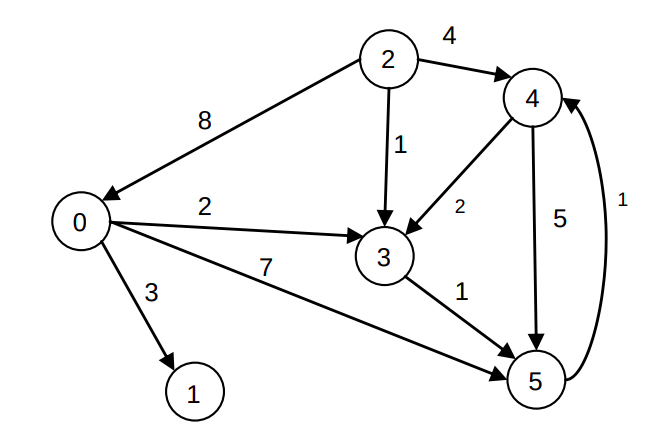
\includegraphics[scale=0.5]{images/graph.png}
	\end{center}
	\captionsetup{justification=centering}
	\caption{Ориентированный взвешенный граф}
	\label{img:graph}
\end{figure}

\subsubsection{Списки смежности}

При представлении графа списками смежности для каждой вершины i хранится список W[i] смежных с ней вершин, как на рисунке \ref{img:graphЦ}.
\begin{figure}[H]
	\begin{center}
		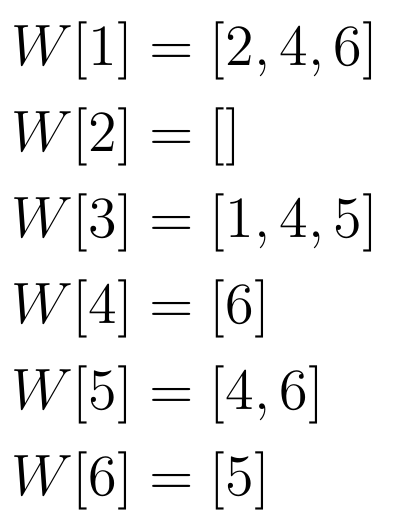
\includegraphics[scale=0.3]{images/matrixW.png}
	\end{center}
	\captionsetup{justification=centering}
	\caption{Матрица смежности}
	\label{img:graphЦ}
\end{figure}

Таким образом, весь граф можно представить одним списком, состоящим из вложенных списков смежности вершин.

\subsubsection{Матрица смежности}

При представлении взвешенного графа матрицей смежности информация о ребрах графа хранится в квадратной матрице, где элемент A[i][j] равен весу ребра, если вершины i и j соединены ребром.  Иначе равен определенному символу (для рассматриваемого графа 0):

\begin{equation}
	A = \begin{pmatrix}
		0 & 3 & 0 & 2 & 0 & 7\\
		0 & 0 & 0 & 0 & 0 & 0\\
		8 & 0 & 0 & 1 & 4 & 0\\
		0 & 0 & 0 & 0 & 0 & 1\\
		0 & 0 & 0 & 2 & 0 & 5\\
		0 & 0 & 0 & 0 & 1 & 0\\
	\end{pmatrix}
\end{equation}

Если граф не является взвешенным, то элемент матрицы смежности равен 1, если вершины соединены.

Матрица смежности требует $O(n^2)$ памяти и может оказаться неэффективным способом хранения дерева или разреженных графов. Но использование матрицы смежности позволяет применять при реализации вычислительных процедур анализа графов матричные алгоритмы обработки данных, которые можно распараллелить. Поэтому при реализации данной лабораторной работы граф будет представляться именно таким образом.

\section{Алгоритм Флойда}

Алгоритм Флойда позволяет найти кратчайшее расстояние между любыми двумя вершинами в графе~\cite{alg}.

\subsection*{Последовательный алгоритм}

Будем считать, что в графе $n$ вершин, пронумерованных числами от $0$ до $n - 1$. Граф задан матрицей смежности, вес ребра $i - j$ равен $w_{ij}$. При отсутствии ребра $i - j$ значение $w_{ij} = -1$, также будем считать, что $w_{ii} = 0$.

Пусть значение $a^k_{ij}$ равно длине кратчайшего пути из вершины $i$ в вершину $j$, при этом путь может заходить в промежуточные вершины только с номерами меньшими $k$ (не считая начала и конца пути). То есть $a^0_{ij}$ - это длина кратчайшего пути из $i$ в $j$, который вообще не содержит промежуточных вершин, то есть состоит только из одного ребра $i - j$, поэтому $a^0_{ij} = w_{ij}$. Значение $a^1_{ij} = w_{ij}$ равно длине кратчайшего пути, который может проходить через промежуточную вершину с номером 0, путь с весом $a^2_{ij}$ может проходить через промежуточные вершины с номерами 0 и 1 и т. д. Путь с весом $a^n_{ij}$ может проходить через любые промежуточные вершины, поэтому значение $a^n_{ij}$ равно длине кратчайшего пути из $i$ в $j$.

Алгоритм Флойда последовательно вычисляет $a^0_{ij}$, $a^1_{ij}$, $a^2_{ij}$, …, $a^n_{ij}$, увеличивая значение параметра $k$. Начальное значение - $a^0_{ij} = w_{ij}$.

Теперь предполагая, что известны значения $a^{k - 1}_{ij}$ вычислим $a^k_{ij}$. Кратчайший путь из вершины $i$ в вершину $j$, проходящий через вершины с номерами, меньшими, чем $k$ может либо содержать, либо не содержать вершину с номером $k - 1$. Если он не содержит вершину с номером $k - 1$, то вес этого пути совпадает с $a^{k - 1}_{ij}$. Если же он содержит вершину $k - 1$, то этот путь разбивается на две части: $i - (k - 1)$ и $(k - 1) - j$. Каждая из этих частей содержит промежуточные вершины только с номерами, меньшими $k - 1$, поэтому вес такого пути равен $a^{k - 1}_{i,k-1} + a^{k - 1}_{k-1,i}$. Из двух рассматриваемых вариантов необходимо выбрать вариант наименьшей стоимости, поэтому:

\begin{equation}
	a^k_{ij} = min(a^{k - 1}_{ij}, a^{k - 1}_{i,k-1} + a^{k - 1}_{k-1,i})
\end{equation}

\subsection*{Параллельный алгоритм}

Параллельный алгоритм Флойда заключается в том, что на k-й итерации мы распределяем k-ю строку между всеми процессами(или потоками), а затем каждый процесс(или поток) выполняет последовательный алгоритм Флойда для полосы матрицы смежности, одновременно обновляя значение матрицы.

